\newpage
\section{Alberi decisionali}
Prendiamo ora un esempio di training set di partite di tennis e costruiamo l'albero decisionale.
\begin{figure}[h!]
    \centering
    \begin{subfigure}{.45\textwidth}
        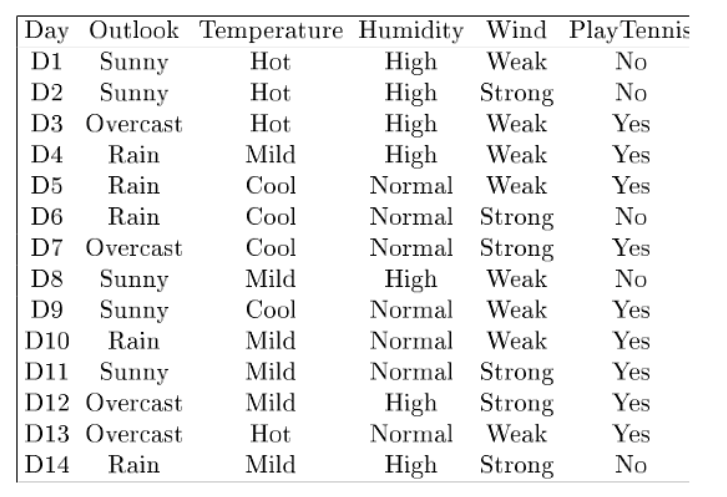
\includegraphics[width=\textwidth]{images/tennis-training-set.png}
    \end{subfigure}
    \begin{subfigure}{.45\textwidth}
        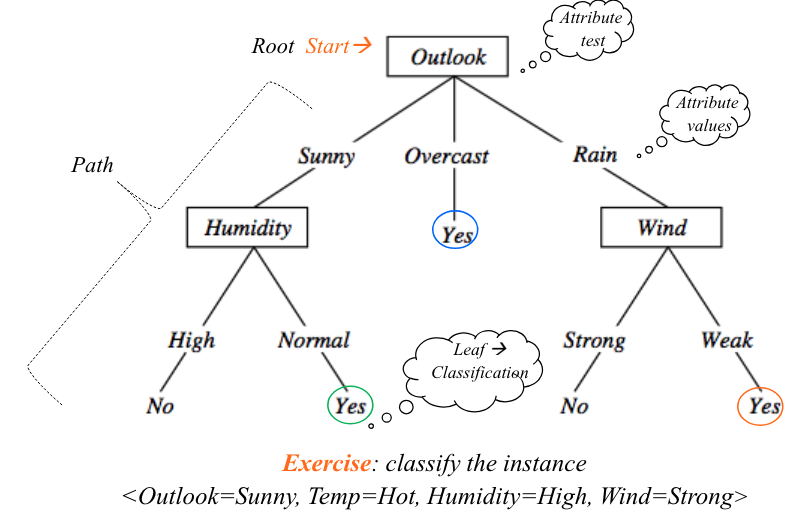
\includegraphics[width=\textwidth]{images/decision-tree-tennis.png}
    \end{subfigure} 
\end{figure}

\hspace{-15pt}Un albero decisionale rappresenta una disgiunzione di congiunzioni di vincoli sul valore
degli attributi.
\begin{enumerate}
    \item (verde) (Outlook = Sunny $\land$ Humidity = Normal) $\land$
    \item (blu) (Outlook = Overcast) $\land$
    \item (rosso) (Outlook = Rain $\land$ Wind = Weak)
\end{enumerate}
H di DT capace di esprimere qualsiasi funzione finita a valori discreti (proposizionale).

\subsection{ID3 algorithm}
ID3 è un algoritmo base per l'apprendimento sui decision tree. Dato un training set di esempi, l'algoritmo per costruire
un decision tree esegue una ricerca nello spazio dei decision tree. La costruzione dell'albero è di tipo \textbf{top-down} e l'algoritmo
esegue una ricerca di tipo \textbf{greedy}.\\\\
La domanda fondamentale è "quale attributo dovrebbe essere testato successivamente? Quale domanda ci dà più informazioni"
\begin{itemize}
    \item Selezionare il \textbf{miglior attributo}
    \item Viene quindi creato un nodo discendete per ogni possibile valore di questo attributo e gli esempi sono suddivisi in base a questo valore.
    \item Il processo viene ripetuto per ogni nodo successore finché tutti gli esempi sono classificati correttamente o non ci sono più attributi.
\end{itemize}
\begin{lstlisting}
    // X: esempi di training
    // T: attributo target
    // Attrs: altri attributi, inizialmente tutti gli attributi
    ID3(X, T, Atter) 
        Create Root Node
        if all X are +: return Root with class +
        if all X are -: return Root with class -
        if Attrs is empty: return Root with class most comon value of T in X
        else 
            A <- best attribute; decision attribute for Root <- A
            for each possible value v_i of A:
                add a new branch bellow Root, for test A = v_i
                X_i <- subset of X con A = v_i
                if X_i is empty then 
                    add a new leaf with class the most common value of T in X
                else then
                    add the subtree generated by ID3(X_i, T, Attr - {A})
        return Root
\end{lstlisting}
Andiamo ad usare la nozione di \textbf{entropia}, comunemente usata nalla teoria dell'informazione.
L'entropia misura l'impurità di una collezione di esempi. Essa dipende dalla distribuzione di una variabile randomica $p$
\begin{itemize}
    \item $S$ è una collezione di esempi di trining.
    \item $p_+$ la proporzioni di esempi positivi in $S$.
    \item $p_-$ la proporzione di esempi negativi in $S$.
\end{itemize}
\begin{definition}
    Definiamo matematicamente \textbf{entropia} come:
    $$Entropy(S) \equiv -p_+ \log_2 p_+ - p_- \log_2p_- \hspace{15pt} [assumento \:\: 0\log_2 0 = 0]$$
\end{definition}
\begin{example}
    Alcuni esempi possono essere i seguenti:
    \begin{itemize}
        \item $Entropy([14+, 0-]) = -14/14\log_2(14/14) - 0\log_2(0) = 0$
        \item $Entropy([9+, 5-]) = -9/14\log_2(9/14) - 5/14\log_2(5/14) = 0.94$
        \item $Entropy([7+, 7-]) = -7/14\log_2(7/14) - 7/14\log_2(7/14) = 1/2 + 1/2 = 1$ questo è un caso con alta inpurità
    \end{itemize}
\end{example}
\begin{note}
    Notare che $0 \leq p \leq 1, 0 \leq entropy \leq 1$
\end{note}
\begin{figure}[h!]
    \centering
    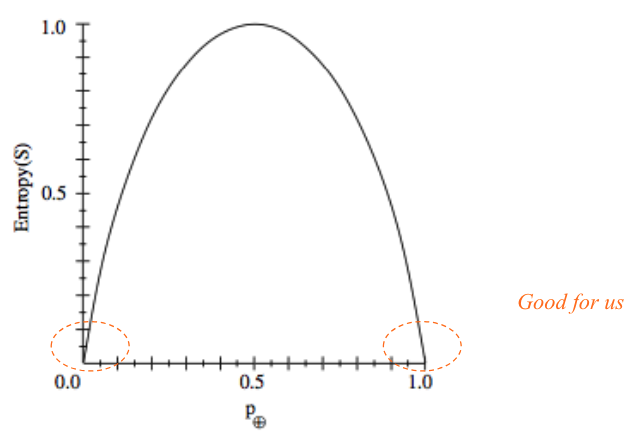
\includegraphics[width=0.5\textwidth]{images/entropia.png}
\end{figure}
Se abbiamo tutti i +1 o tutti i -1 allora abbiamo 0 entropia cioè "no informazioni". Il massimo per $S$ la abbiamo invece con esempi 1/2+ e 1/2-.\\\\
Il guadagno di informazioni è la riduzione prevista dell'entropia causata partizionando gli esempi su un attributo. 
\begin{definition}
    Definiamo la \textbf{Riduzione attesa dell’entropia conoscendo A}
    $$Gain(S, A) = Entrpy(S) - \sum_{v \in Values(A)}\frac{|Sv|}{S}Entropy(Sv)$$
    Dove $values(A)$ sono i possibili valori per A, mentre $Sv$ è un sottoinsieme di esempi di S per i quali A ha valore v (somma di pesi)
\end{definition}
\hspace{-15pt}Maggiore è il guadagno di informazione, più efficace è l'attributo classificazione dei dati di addrestramento (maggiore variazione nell'omogeneità dei distribuzione delle classi nei sottoinsiemi, massima separazione delle classi).
\textbf{Omogeneo}, poiché [14+, 0-] o [0+,7-] ci consentono una classificazione “chiara”.\\\\
L'entropia misura l'omogeneità (anzi impurità) della classe del sottoinsieme di esempi, quindi: \textbf{Selezionare A che massimizzi}
$$Gain(S, A) = Entropy(S) - \sum_{v \in Values(A)} \frac{|Sv|}{|S|} Entropy(Sv)$$
Dopo la suddivisione, valori più bassi (obiettivi più omogenei) in ciascun sottoinsieme porta ad un guadagno più elevato.
Lo scopo è quello di separare gli esempi in base al target, trovare l'attributo che discimina gli esempi a cui appartengono diverse classi target.
\begin{figure}[h!]
    \centering
    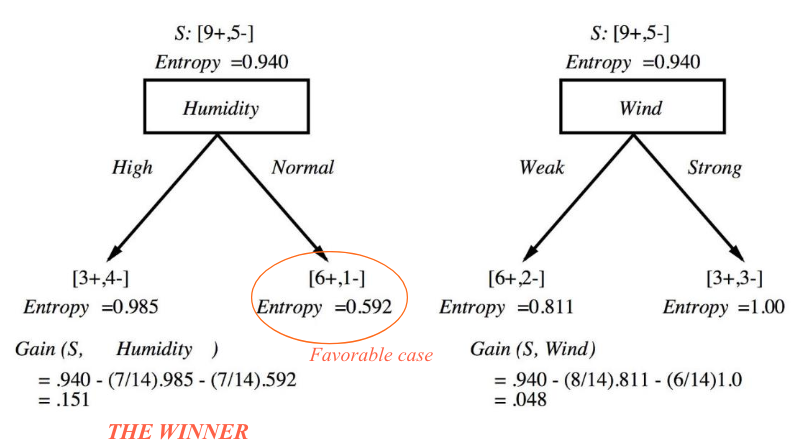
\includegraphics[width=0.6\textwidth]{images/esempio-select-best-attribute.png}
\end{figure}

\begin{minipage}{0.65\linewidth}
    Il guadagno di informazioni favorisce attributi con molti valori possibili. Consideriamo l'attributo "Date" nell'esempio "PlayTennis".\\\\
    "Date" ha il massimo guadagno di informazioni. Ogni giorno corrisponde ad un sottoinsieme differente che è puro: $[1+, 0-]$ o $[0+, 1-] \to 0$ entropia. 
    Abbiamo un adattamento perfetto (separazione) dei dati di trining, ma non è significato: non serve per i casi invisibili. \\\\
    Chiediamoci ora come evitare la generazione di molti piccoli
    sottoinsiemi?    
\end{minipage}
\hfill
\begin{minipage}{0.35\linewidth}
    \centering
    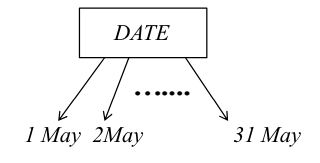
\includegraphics[width=0.95\textwidth]{images/problem-information-gain.png}
\end{minipage}
\begin{definition}
    Definiamo quello che è chiamato \textbf{gain ratio}
    $$GainRation(S, A) = \frac{Gain(S, A)}{SplitInInformation(S, A)}$$
    Dove abbiamo che:
    $$SplitInInformation(S, A) = -\sum_{i=1}^{C}\frac{|S_i|}{|S|} \log_2\frac{|S_i|}{|S|}$$
\end{definition}
\hspace{-15pt}Abbiamo che $S_1$ sono degli insiemi ottenuti partizionando sul valore $v_i$ di $A$ finao al valore $c$.
SplitInInformation misura l'entropia di S rispetto ai valori di A, Più i dati sono distribuiti uniformamente, più sono alti.\\\\
Il GainRation penalizza gli attributi che dividono gli esempi in molte piccole classi come per Date.
Sia $|S| = n$ la divisione degli esempi di date in $n$ sottoinsiemi.
$$SplitInInformation(S, Date) = -[(1(n/\log_2 1/n)) + \dots + (1/2 \log_2 1/n)] = -\log_2 1/n = \log_2$$
Il quale è $> 1$ per $n > 2$ quindi riduciamo il GainRatio.\\
Confronto con un A che divide i dati in due classi pari (con $(n/2)/n = 1/2$):
$$SplitInInformation(S, A) = -[(1/2 \log_2 1/2) + (1/2\log_2 1/2)] = -[-1/2 - 1/2] = 1 \to \text{ no reduction }$$
Abbiamo un problema: $SplitInInformation(S, A)$ può essere zero o molto piccolo quando $|S_i|\approx |S|$ per qualche valore $i \: [\log 1 = 0]$.
Per mitigare questo effetto, vengono usate le seguenti euristiche:
\begin{enumerate}
    \item Calcolare $Gain$ per ogni attributo.
    \item Applicare $GainRation$ solo per gli attributi con $Gain$ sopra la media.
\end{enumerate} 